\documentclass[12pt]{article}

\input{setup.tex}

\begin{document}

\begin{large}
\noindent AMS 206B -- Exam 2
\smallskip

\noindent Mickey Warner
\end{large}
\bigskip

\noindent We fit a data set with $I=5$ time series and $T=300$ observations each. The AR(1) model is given by
\begin{eqnarray*}
y_{t,i} &=& \phi_iy_{t-1,i}+\epsilon_{t,i},~~~\epsilon_{t,i}\sim N(0, \nu), \\
\phi_i|\phi &\overset{iid}\sim& N(\phi, \tau^2), \\
p(\phi,\nu) &\propto& 1/\nu
\end{eqnarray*}
\noindent with $\tau^2=0.1$. The full likelihood is given by the $I$ products of
\[ p(y_{1:T,i}|\phi_i,\nu) = \frac{(1-\phi_i^2)^{1/2}}{(2\pi\nu)^{T/2}}\exp\left\{-\frac{1}{2\nu}\left[y_{1,i}^2(1-\phi_i^2)+\sum_{t=2}^T(y_{t,i}-\phi_iy_{t-1,i})^2\right]\right\}. \]
\noindent This expression can be simplified by approximating it with the conditional likelihood given by
\[ p(y_{2:T,i}|\phi_i,\nu,y_{1,i}) = \frac{1}{(2\pi\nu)^{T/2}}\exp\left\{-\frac{1}{2\nu}\sum_{t=2}^T(y_{t,i}-\phi_iy_{t-1,i})^2\right\}. \]
\noindent The approximation is more accurate as $T$ increases since the first observation $y_{1,i}$ places less and less of a role in the estimation process. We sample from the posterior using both likelihoods and compare these results and approaches. We also look at how choices for $\tau^2$ affect our posterior results.
\bigskip

\noindent A plot of the data is given in Figure \ref{data}.
\begin{figure}[H]
\begin{center}
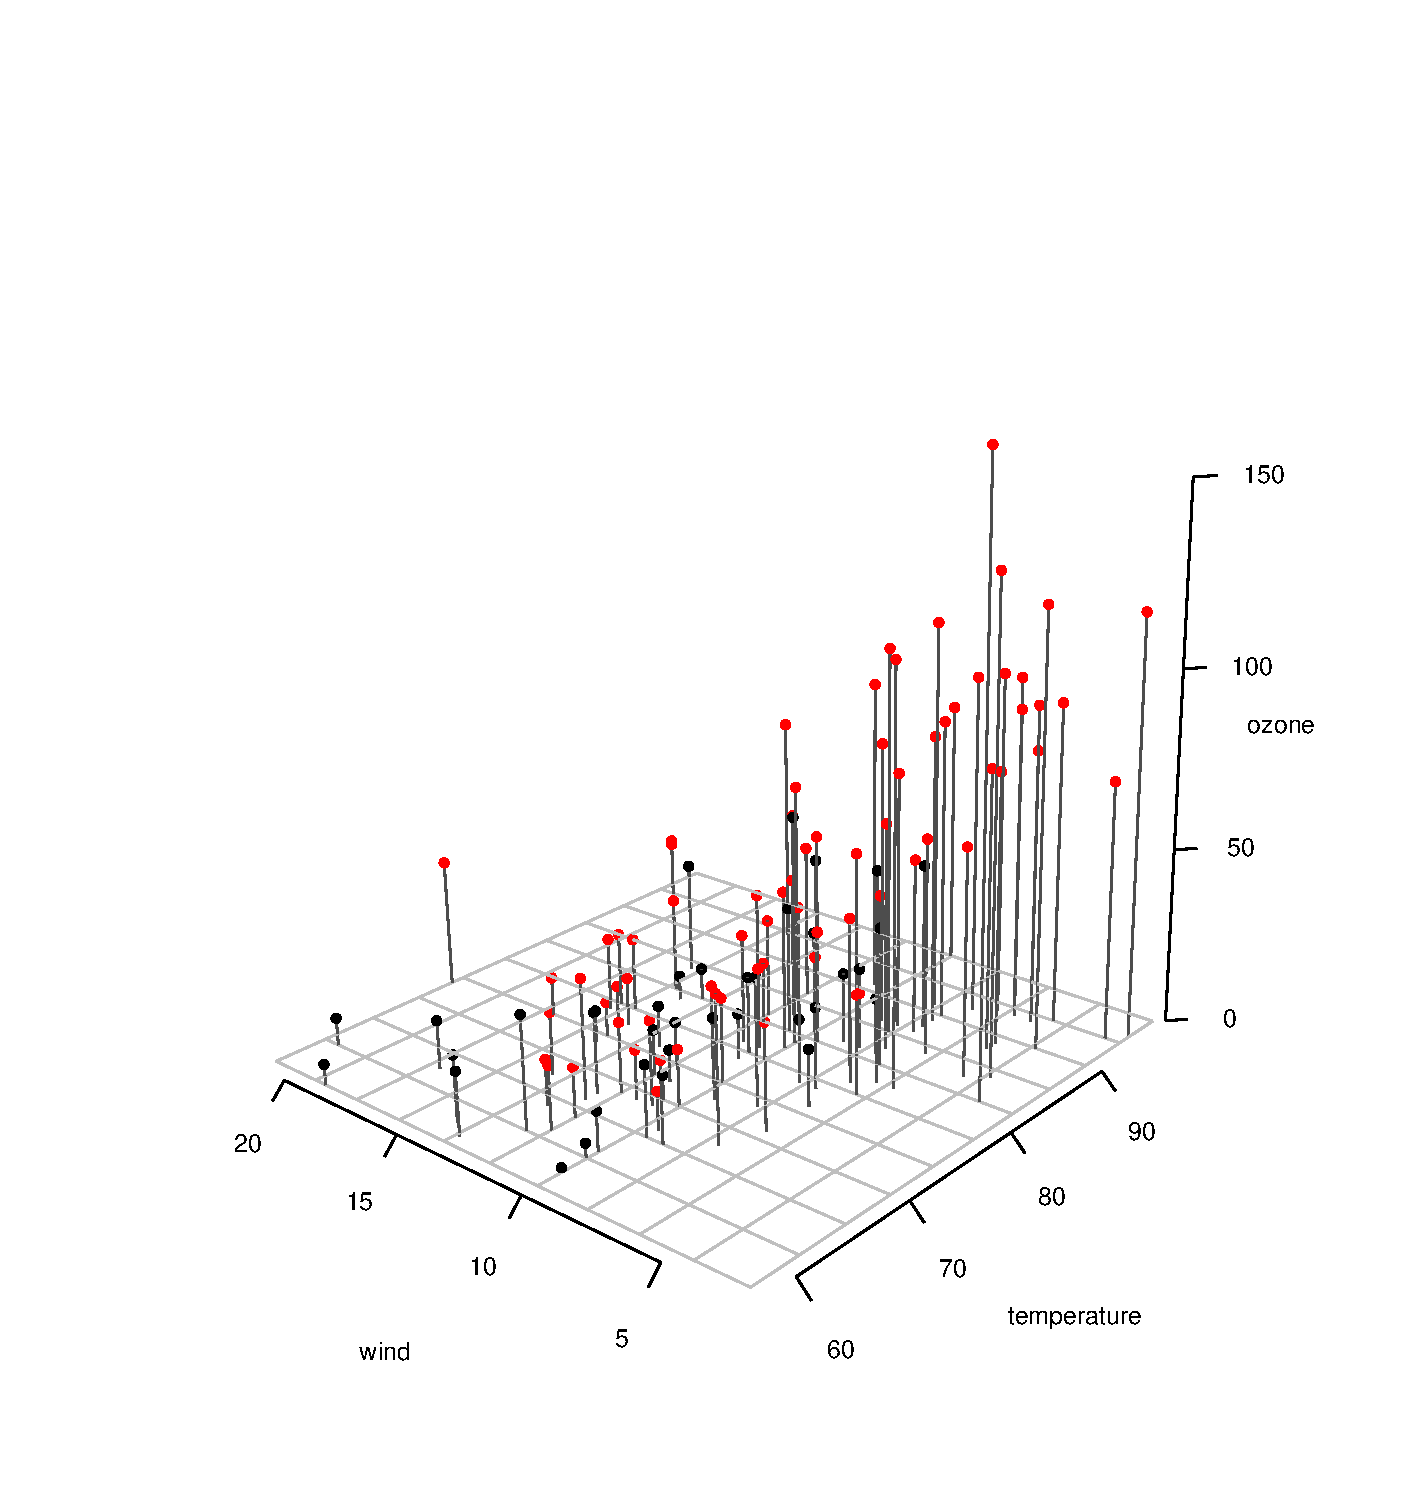
\includegraphics[scale=0.38]{figs/data.pdf}
\end{center}
\caption{The $I=5$ time series, each with $T=300$ observations.}
\label{data}
\end{figure}

\section{Posterior based on conditional likelihood}

\noindent Denote $\m{y}$ as the time series data. We obtain samples using Gibbs updates from the full conditionals of each parameter. These are given by:
\begin{eqnarray*}
\nu|\phi_1,\ldots,\phi_I,\phi,\m{y} &\sim& IG\left(\frac{IT}{2}, \frac{1}{2}\sum_{i=1}^I\left[\sum_{t=2}^T(y_{t,i}-\phi_iy_{t-1,i})^2\right]\right) \\
\phi_i|\phi_{-i},\phi,\nu,\m{y} &\sim& N\left(\frac{\tau^2\sum_{t=2}^Ty_{t,i}y_{t-1,i} + \nu\phi}{\tau^2\sum_{t=2}^Ty_{t-1,i}^2 + \nu},\frac{\tau^2\nu}{\tau^2\sum_{t=2}^Ty_{t-1,i}^2 + \nu}\right) \\
\phi|\phi_1,\ldots,\phi_I,\nu,\m{y} &\sim& N\left(\frac{1}{I}\sum_{i=1}^I\phi_i, \frac{\tau^2}{I}\right),
\end{eqnarray*}
\noindent where $\phi_{-i}$ denotes the vector of $(\phi_1,\ldots,\phi_I)$ excepting the $i$th element. These are easy to sample from using standard methods. After a burn-in of $5000$ draws, we keep $20000$ samples to calculate density estimates and other functionals. Density estimates of the posterior samples are shown in Figure \ref{posts_1} and a numerical summary is given in Table \ref{summ1}.

\section{Posterior based on full likelihood}

\noindent When using the full likelihood, a small adjustment is made to the full conditional of $\nu$ and Metropolis steps are used to draw $\phi_i$. This leaves us with closed-form expressions for $\nu$ and $\phi$, but not for $\phi_i$:
\begin{eqnarray*}
\nu|\phi_1,\ldots,\phi_I,\phi,\m{y} &\sim& IG\left(\frac{IT}{2}, \frac{1}{2}\sum_{i=1}^I\left[y_{1,i}^2(1-\phi_i^2)+\sum_{t=2}^T(y_{t,i}-\phi_iy_{t-1,i})^2\right]\right) \\
p(\phi_i|\phi_{-i},\phi,\nu,\m{y}) &\propto& (1-\phi_i^2)^{1/2}\exp\left\{-\frac{1}{2\nu}\left[y_{1,i}^2(1-\phi_i^2)+\sum_{t=2}^T(y_{t,i}-\phi_iy_{t-1,i})^2\right]\right\}\times \\
& & ~~~~ ~~~~ \exp\left\{-\frac{1}{2\tau^2}(\phi_i-\phi)^2\right\} \\
\phi|\phi_1,\ldots,\phi_I,\nu,\m{y} &\sim& N\left(\frac{1}{I}\sum_{i=1}^I\phi_i, \frac{\tau^2}{I}\right).
\end{eqnarray*}
\noindent This formulation necessarily requires $\phi_i\in[-1,1]$; we define $p(\phi_i,\phi_{-1},\phi,\nu,\m{y})=0$ outside of this interval. We use normal proposal distributions for the Metropolis updates and each are tuned individually to get desirable acceptance rates.
\bigskip

\noindent Results are shown in Figure \ref{posts_2} and Table \ref{summ2}.

\begin{figure}[H]
\begin{center}
\includegraphics[scale=0.60]{figs/posts_1.pdf}
\end{center}
\caption{\emph{Conditional likelihood.} Kernel density estimates of the posterior for each parameter (marginally). Top: the posterior for $\nu$. Bottom: posteriors for the group mean $\phi$ (black) and the individual autoregressive parameters (colored).}
\label{posts_1}
\end{figure}

\begin{table}[H]
\begin{center}
\begin{tabular}{rrrrr}
    \hline
 & mean & sd & 2.5\% & 97.5\% \\ 
    \hline
$\nu   $ & 1.07 & 0.04 & 0.99 & 1.15 \\ 
$\phi_1$ & 0.94 & 0.02 & 0.90 & 0.98 \\ 
$\phi_2$ & 0.98 & 0.01 & 0.96 & 1.00 \\ 
$\phi_3$ & 0.59 & 0.05 & 0.49 & 0.68 \\ 
$\phi_4$ & 0.64 & 0.04 & 0.56 & 0.72 \\ 
$\phi_5$ & 0.85 & 0.03 & 0.79 & 0.91 \\ 
$\phi  $ & 0.80 & 0.14 & 0.52 & 1.08 \\ 
    \hline
\end{tabular}
\end{center}
\caption{\emph{Conditional likelihood.} Summary statistics from the posterior samples. Sample means, standard deviations, and equal-tailed 95\% probability intervals are given.}
\label{summ1}
\end{table}

\begin{figure}[H]
\begin{center}
\includegraphics[scale=0.60]{figs/posts_2.pdf}
\end{center}
\caption{\emph{Full likelihood.} Kernel density estimates of the posterior for each parameter (marginally). Top: the posterior for $\nu$. Bottom: posteriors for the group mean $\phi$ (black) and the individual autoregressive parameters (colored).}
\label{posts_2}
\end{figure}

\begin{table}[H]
\begin{center}
\begin{tabular}{rrrrrrr}
  \hline
 & mean & sd & 2.5\% & 97.5\% & ar & effSize \\ 
  \hline
$\nu   $ & 1.07 & 0.04 & 1.00 & 1.15 & --- & --- \\ 
$\phi_1$ & 0.94 & 0.02 & 0.90 & 0.98 & 0.27 & 3417.27 \\ 
$\phi_2$ & 0.98 & 0.01 & 0.96 & 1.00 & 0.26 & 3171.56 \\ 
$\phi_3$ & 0.59 & 0.05 & 0.49 & 0.68 & 0.28 & 3672.59 \\ 
$\phi_4$ & 0.64 & 0.04 & 0.56 & 0.73 & 0.28 & 3523.27 \\ 
$\phi_5$ & 0.85 & 0.03 & 0.79 & 0.91 & 0.28 & 3762.62 \\ 
$\phi  $ & 0.80 & 0.14 & 0.52 & 1.08 & --- & --- \\ 
   \hline
\end{tabular}
\end{center}
\caption{\emph{Full likelihood.} Summary statistics from the posterior samples. Sample means, standard deviations, equal-tailed 95\% probability intervals, and Metropolis acceptance rate and effective sample size (when applicable) are given.}
\label{summ2}
\end{table}

\section{Comparison between the two approaches}

\noindent Figures \ref{posts_1} and \ref{posts_2} show very similar results. The only difference (though not seen from the figures) is that the conditional likelihood approach resulted in samples for $\phi_1$ and $\phi_2$ being greater than 1. This is impossible for the full likelihood approach and also causes some issues with autoregressive models. The summary statistics in both cases are nearly identical.
\bigskip

\noindent Since the conditional likelihood approximates the full likelihood, it isn't any surprise that the posteriors in each case are so similar. The main difference then is in the approach itself. Do we prefer an easier way to obtain samples over having a more accurate posterior? Or are we fine dealing with the challenges involved with the Metropolis algorithm?
\bigskip

\noindent For this data set, the Metropolis updates performed fairly well. We had no apparent issues in convergence or finding good proposal distributions. One area of concern is the effective sample size: out of 20000 iterations, we had in effect only 3500 samples from the posterior. Should the data set grow (considerably) in size, we may not have the resources to obtain a sufficient number of draws.

\section{Prior sensitivity analysis}

\noindent We repeat both analyses for $\tau^2=1$ and $\tau^2=10$ (recall the above results are for $\tau^2=0.1$). The parameter $\tau^2$ is the prior variance that describes how each $\phi_i$ differs from the population mean $\phi$.
\bigskip

\noindent The full conditionals given in Sections 1 and 2 reveal how much of a role $\tau^2$ plays in the posterior. For $\phi$, $\tau^2$ interacts with the data only through the number of time series $I$, thus being more influential to the posterior of $\phi$. For each $\phi_i$, $\tau^2$ can affect both the mean and variance, but it can also be swamped out by the data more easily. For $\nu$, the affect of $\tau^2$ only manifests itself by changes made to $\phi_1,\ldots,\phi_I$.
\bigskip

\noindent How $\tau^2$ affects the posteriors can be seen in the figures on the next two pages. Figures \ref{posts1b} and \ref{posts2b} compare the conditional likelihood approach with the full likelihood approach, respectively. Again, the two posteriors are very similar. Compared to Figures \ref{posts_1} and \ref{posts_2}, we see that the only difference is found in $\phi$. For $\tau^2=1$, the posterior for $\phi$ has a much higher variance while the other parameters remain the same.
\bigskip

\noindent Figures \ref{posts1c} and \ref{posts2c} show posterior density estimates for $\tau^2=10$. We again see a wider $\phi$ (almost unseen in the figures) while $\phi_1,\ldots,\phi_I,\nu$ remain the same.

\newpage 

\begin{figure}[H]
\begin{center}
\includegraphics[scale=0.45]{figs/posts_1b.pdf}
\end{center}
\caption{\emph{Conditional likelihood.} Posterior distributions for $\tau^2=1$.}
\label{posts1b}
\end{figure}

\begin{figure}[H]
\begin{center}
\includegraphics[scale=0.45]{figs/posts_2b.pdf}
\end{center}
\caption{\emph{Full likelihood.} Posterior distributions for $\tau^2=1$.}
\label{posts2b}
\end{figure}

\begin{figure}[H]
\begin{center}
\includegraphics[scale=0.45]{figs/posts_1c.pdf}
\end{center}
\caption{\emph{Conditional likelihood.} Posterior distributions for $\tau^2=10$.}
\label{posts1c}
\end{figure}

\begin{figure}[H]
\begin{center}
\includegraphics[scale=0.45]{figs/posts_2c.pdf}
\end{center}
\caption{\emph{Full likelihood.} Posterior distributions for $\tau^2=10$.}
\label{posts2c}
\end{figure}

\end{document}
